\section{Different Types of Pose Maps}

\begin{figure*}[h]
    \centering
    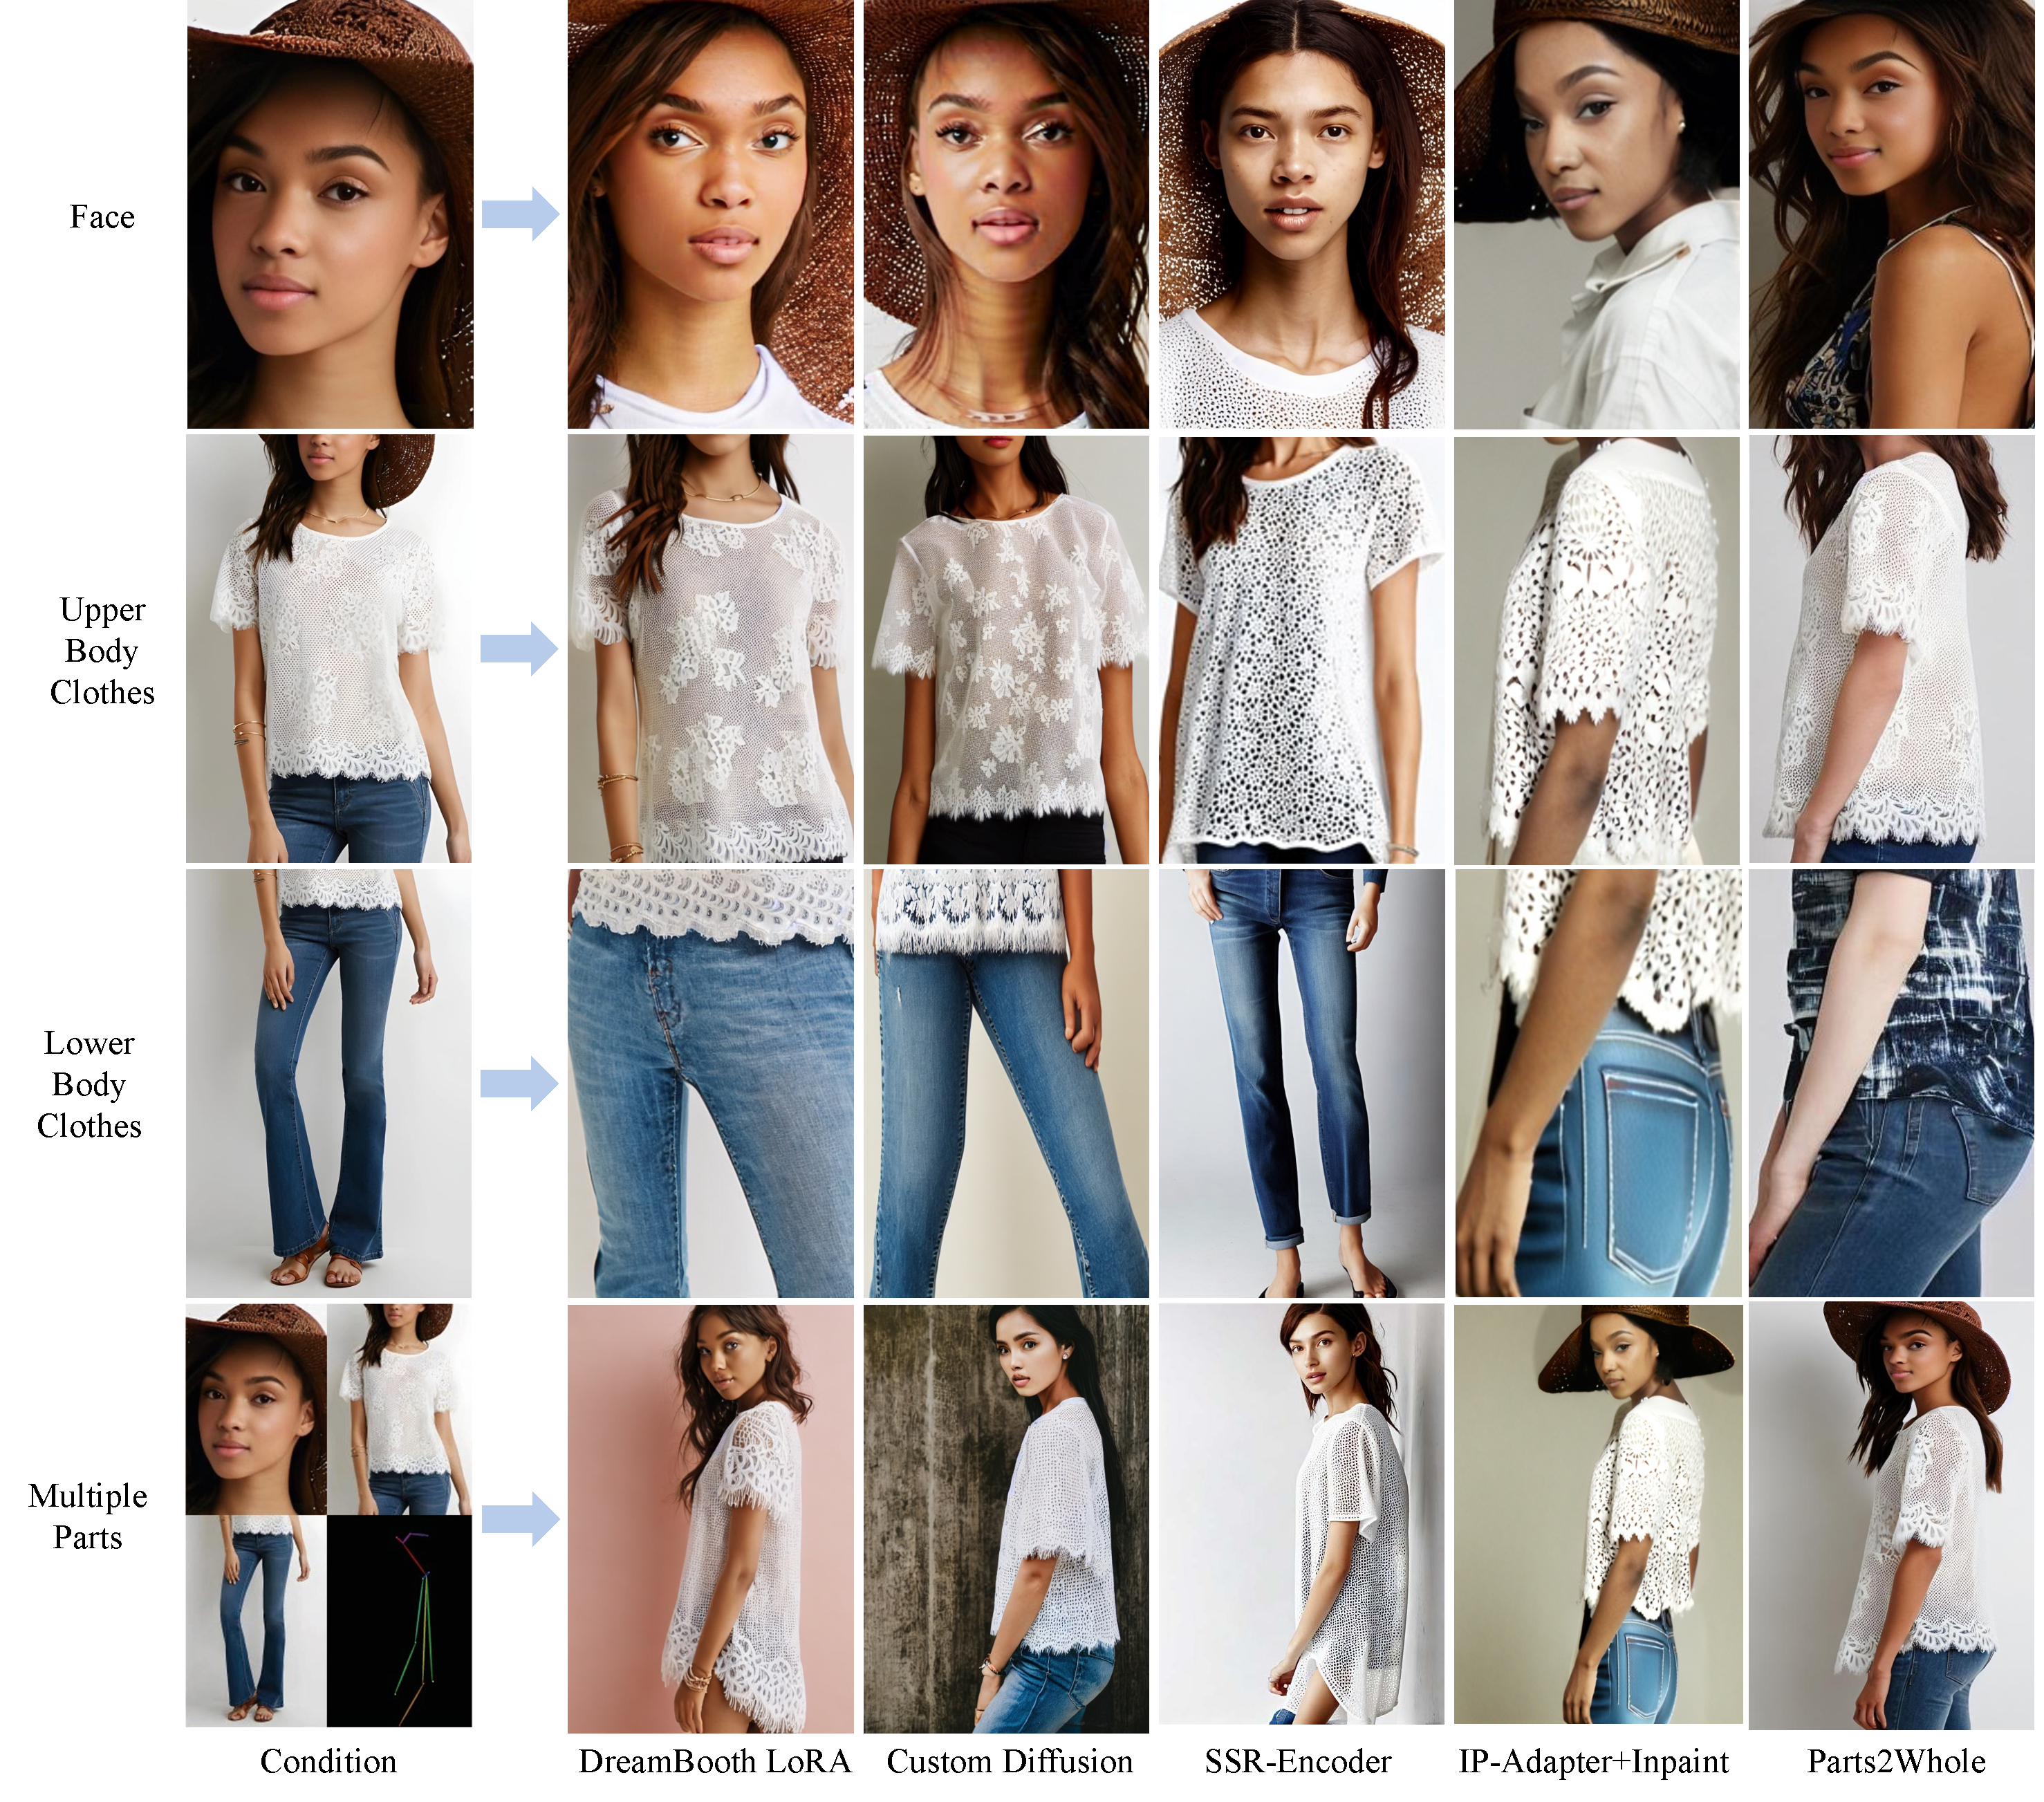
\includegraphics[width=1\textwidth]{figure/supp_existing_work.pdf}
    \caption{Results of single-condition and multi-condition generation. The top three rows labeled ``face'', ``upper body clothes'', ``lower body clothes'' represent separate conditions. The fourth row demonstrates joint control under multi-part conditions.}
    \label{fig:existing_methods}
\end{figure*}

To show the ability of Parts2Whole to generate human image conditions on different types of pose maps, we train a new Parts2Whole model but with \textbf{OpenPose} as a condition. As shown in \cref{fig:supp_openpose}, the generated images strictly maintain consistency with the target pose, and each body part retains the appearance information from the reference images.







